\graphicspath{{./images/bmps/}{./images/vects/}{./images/}
  {./images/presentation/bmps/}{./images/presentation/vects/}{./images/presentation/}
  {./images/chapter00/bmps/}{./images/chapter00/vects/}{./images/chapter00/}
  {./images/chapter01/bmps/}{./images/chapter01/vects/}{./images/chapter01/}
  {./images/chapter02/bmps/}{./images/chapter02/vects/}{./images/chapter02/}
  {./images/chapter03/bmps/}{./images/chapter03/vects/}{./images/chapter03/}
  {./images/chapter04/bmps/}{./images/chapter04/vects/}{./images/chapter04/}
  {./images/chapter05/bmps/}{./images/chapter05/vects/}{./images/chapter05/}
  {./images/chapter06/bmps/}{./images/chapter06/vects/}{./images/chapter06/}
  {./images/chapter07/bmps/}{./images/chapter07/vects/}{./images/chapter07/}
}

\section{Introduction}
  \begin{frame}{Introduction}
    \begin{itemize}
      \item<1-> Humans should not drive.
      \begin{itemize}
	\item<2-> Road injuries are one of the top-ten causes death, according to the World Health Organization (WHO).
	\note {Fortunately, the number of deaths for this cause has been reduced.}
	\note {Popularization of Advanced Driver Assistance Systems (ADAS) could be very related to this fact.}
	\item<3-> Driving is difficult, too.
	\note{An average US citizen expends 38 hours stuck in traffic.}
      \end{itemize}
      \item<4-> The amount of research related to autonomous vehicles has increased a lot.
    \end{itemize}  
    \begin{center}
      \includegraphics<1-1>[height=.5\textheight]{CarCartoon}
      \includegraphics<2-2>[height=.5\textheight]{WHO-data-10-deaths}
      \includegraphics<3-3>[height=.5\textheight]{trafficsigns}
      \includegraphics<4-4>[height=.5\textheight]{uav_research}
    \end{center}
  \end{frame}
  
  \begin{frame}{Advantages of autonomous vehicles}
    \begin{columns}[c] % the "c" option specifies center vertical alignment
      \column{.5\textwidth} % column designated by a command
      \begin{itemize}
	\item<1-> Higher safety.      
	\item<2-> Reduced traffic congestion.
	\item<3-> More free time.
	\item<4-> Higher speed limits.
	\item<5-> Occupant constraints.
	\item<6-> Parking problems.
	\item<7-> Traffic police.
	\item<8-> Vehicle insurance.
	\item<9-> Road signs.
	\item<10-> Smoother ride.
      \end{itemize}  
      \column{.5\textwidth}
      \begin{center}
	\includegraphics<1-1>[width=\textwidth]{safety}
	\includegraphics<2-2>[width=\textwidth]{congestion}
	\includegraphics<3-3>[width=\textwidth]{freetime}
	\includegraphics<4-4>[width=\textwidth]{speedlimit}
	\includegraphics<5-5>[width=\textwidth]{stpatricks}
	\includegraphics<6-6>[width=\textwidth]{parking}
	\includegraphics<7-7>[width=\textwidth]{police}
	\includegraphics<8-8>[width=\textwidth]{insurance}
	\includegraphics<9-9>[width=\textwidth]{roadsign}
	\includegraphics<10-10>[width=0.8\textwidth]{smoothride}
      \end{center}
    \end{columns}
    
    \note {
    \begin{itemize}
      \item As said, higher safety due a to a decrease in the number of traffic accidents.
      \item Reduced traffic congestion, as the roads can increase their capacity.
      \item Vehicle occupants can spend their time in things other than driving.
      \item Higher speed limits.
      \item Occupants are not tied to constraints like being under age, blind, intoxicated, etc.
      \item Alleviation of parking scarcity and reduction of space required for vehicle parking.
      \item Reduction in the need for traffic police and vehicle insurance.
      \item Physical road signs will not be needed anymore: autonomous cars could receive necessary communication electronically.
      \item Smoother ride.
    \end{itemize}
    }
  \end{frame}

  \subsection{Problem Statement}
  \begin{frame}{Problem Statement}
    \begin{itemize}
     \item<1-> We propose different methods which will be used for the detection and tracking of obstacles by our prototype, Verdino.
     \item<2-> These will be used by a global and a local planner for generating and following a safe path.
    \end{itemize}
    \begin{center}
      \includegraphics<1->[height=.4\columnwidth]{verdino}
    \end{center}
  \end{frame}
  
  \begin{frame}{Pipeline}
    \begin{center}
      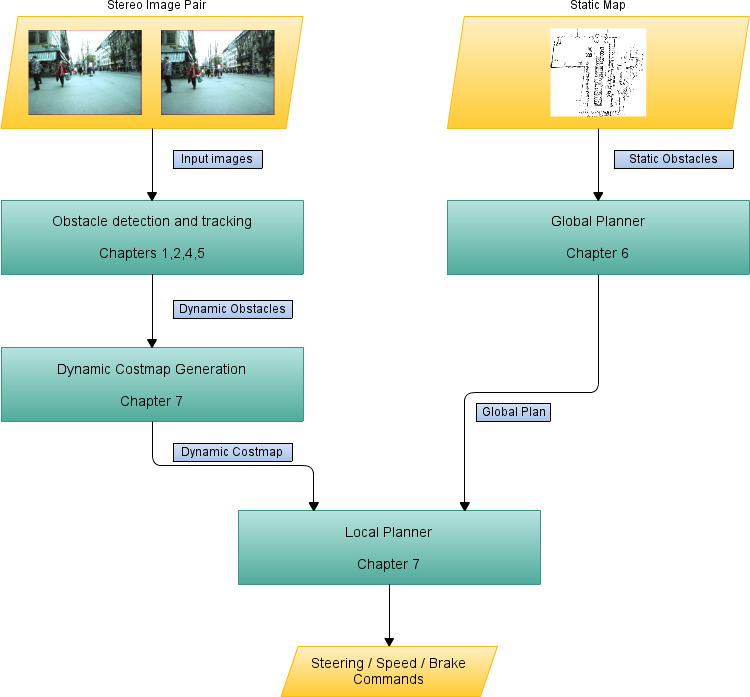
\includegraphics{pipeline_cp0}
    \end{center}
    
  \end{frame}

  
  \begin{frame}{Obstacle detection and tracking}
    \begin{itemize}
    \item<1-> Goals:
      \begin{enumerate}
      \item<2-> Good obstacle detection rate. 
      \item<3-> Obstacle localization.
      \item<4-> Real time.
      \item<5-> Environment conditions independence.
      \item<6-> Tracking capabilities.
      \item<7-> Moving cameras.
      \end{enumerate}
    \end{itemize}
  \end{frame}
  
  \begin{frame}{Obstacle detection and tracking}
    \begin{itemize}
      \item <1-> We propose four different approaches:
      \begin{enumerate}
	\item<1-> Change detection and image registration. 
	\item<2-> Background substraction and nonrigid point set registration.
	\item<3-> Stixels.
	\item<4-> Voxels and a particle filter.
      \end{enumerate}
    \end{itemize}
      
    \begin{center}
      \includegraphics<1-1>[height=.3\columnwidth]{database}
      \includegraphics<2-2>[height=.3\columnwidth]{fig6}
      \includegraphics<3-3>[height=.3\columnwidth]{stixels_over_original}
      \includegraphics<4-4>[height=.3\columnwidth]{fakePointCloud}
    \end{center}
  \end{frame}
  
  \begin{frame}{Obstacle Avoidance and Planning}
    We distinguish two different levels:
    \begin{enumerate}
     \item<1-> Global planning. 
     \item<2-> Local planning.
    \end{enumerate}

    \begin{center}
      \includegraphics<1-1>[height=.35\columnwidth]{figure7}
      \includegraphics<2-2>[height=.35\columnwidth]{example3a}
    \end{center}
  \end{frame}
  
  \begin{frame}{Evaluation of Stereo 3D Reconstruction Algorithms}
    Apart from the previous, we developed some methods intended to assess the performance of the 3D stereo reconstruction algorithms used for the particle filter based approach.
    
    \begin{center}
      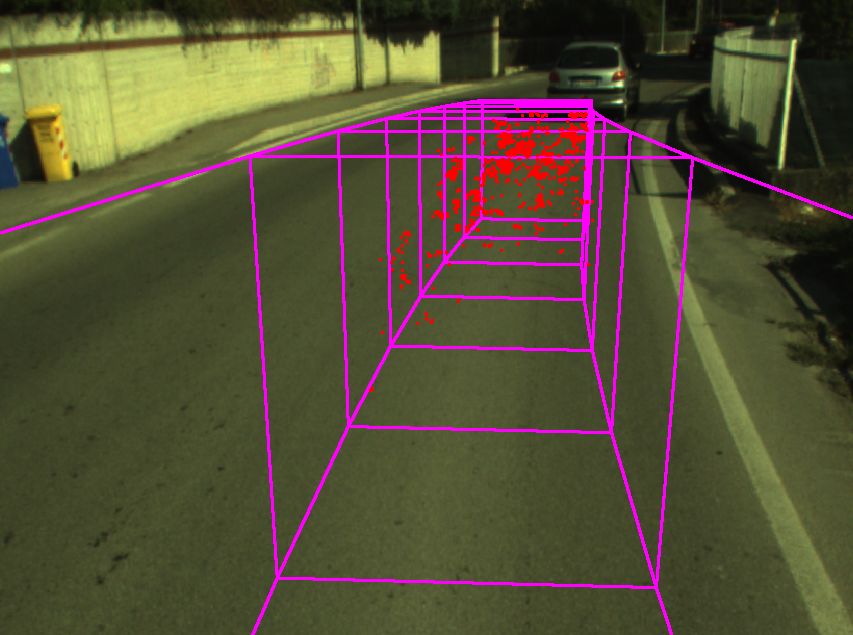
\includegraphics[height=.4\columnwidth]{fc}
    \end{center}
    
  \end{frame}
    
  \subsection{Previous Work}
  \begin{frame}{Autonomous vehicles review}
    \begin{columns}[T] % the "c" option specifies center vertical alignment
      \column{.5\textwidth} % column designated by a command
      \footnotesize
      \begin{itemize}
	\item<1-> \textbf{(1987-1995)} EC EUREKA Prometheus Project.
	\item<2-> \textbf{(1996)} ARGO Project.
	\item<3-> \textbf{(2004)} $1^{st}$ DARPA's Grand Challenge.
	\item<4-> \textbf{(2005)} $2^{nd}$ DARPA's Grand Challenge.
	\item<5-> \textbf{(2007)} DARPA's Urban Challenge.
	\item<6-> \textbf{(2010, 2012, 2013)} Korean Autonomous Vehicle Competition (AVC).
      \end{itemize}  
      \column{.5\textwidth}
      \begin{center}
	\vskip -1cm
       	\begin{overlayarea}{\textwidth}{\textheight}
	  \only<1>{
	  \begin{block}{EC EUREKA Project}
	    \begin{itemize}
	    \item VITA-2\\
	    \begin{center}\includegraphics<1->[width=0.5\textwidth]{vita2}\end{center}
	    \item VaMP\\
	    \begin{center}\includegraphics<1->[width=0.5\textwidth]{VaMP}\end{center}
	    \end{itemize}
	  \end{block}
	  }
	  \only<2>{
	  \begin{block}{ARGO Project}
	    \begin{itemize}
	      \item Lancia Thema.
	      \item Follow the lane marks of a road.
	      \item 1,900\,km
	      \item Average of 60\,Km/h.
	    \end{itemize}
	    \begin{center}\includegraphics<1->[width=0.5\textwidth]{argo}\end{center}
	  \end{block}
	  }
	  \only<3>{
	  \begin{block}{$1^{st}$ DARPA's Grand Challenge}
	    \begin{itemize}
	      \item Mojave Desert.
	      \item 240\,km route.
	      \item Listing of check points.
	      \item None finished the route.
	    \end{itemize}
	    \begin{center}\includegraphics<1->[width=0.5\textwidth]{urbanchallenge2004}\end{center}
	  \end{block}
	  }
	  \only<4>{
	  \begin{block}{$2^{nd}$ DARPA's Grand Challenge}
	    \begin{figure}[t]
		    \centering
		    \begin{subfigure}[b]{0.4\textwidth}
		      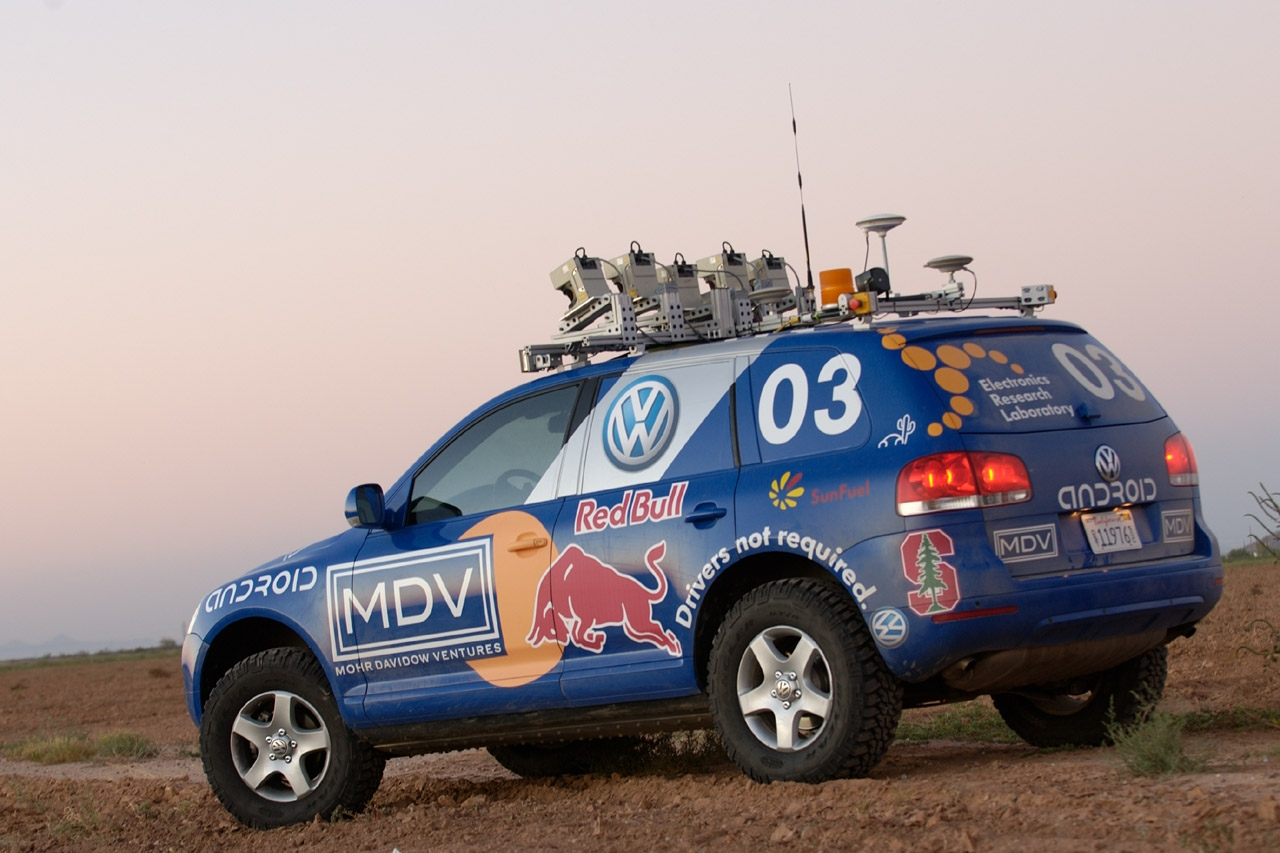
\includegraphics[width=\textwidth]{stanley}
		    \end{subfigure}
		    ~
		    \begin{subfigure}[b]{0.4\textwidth}
		      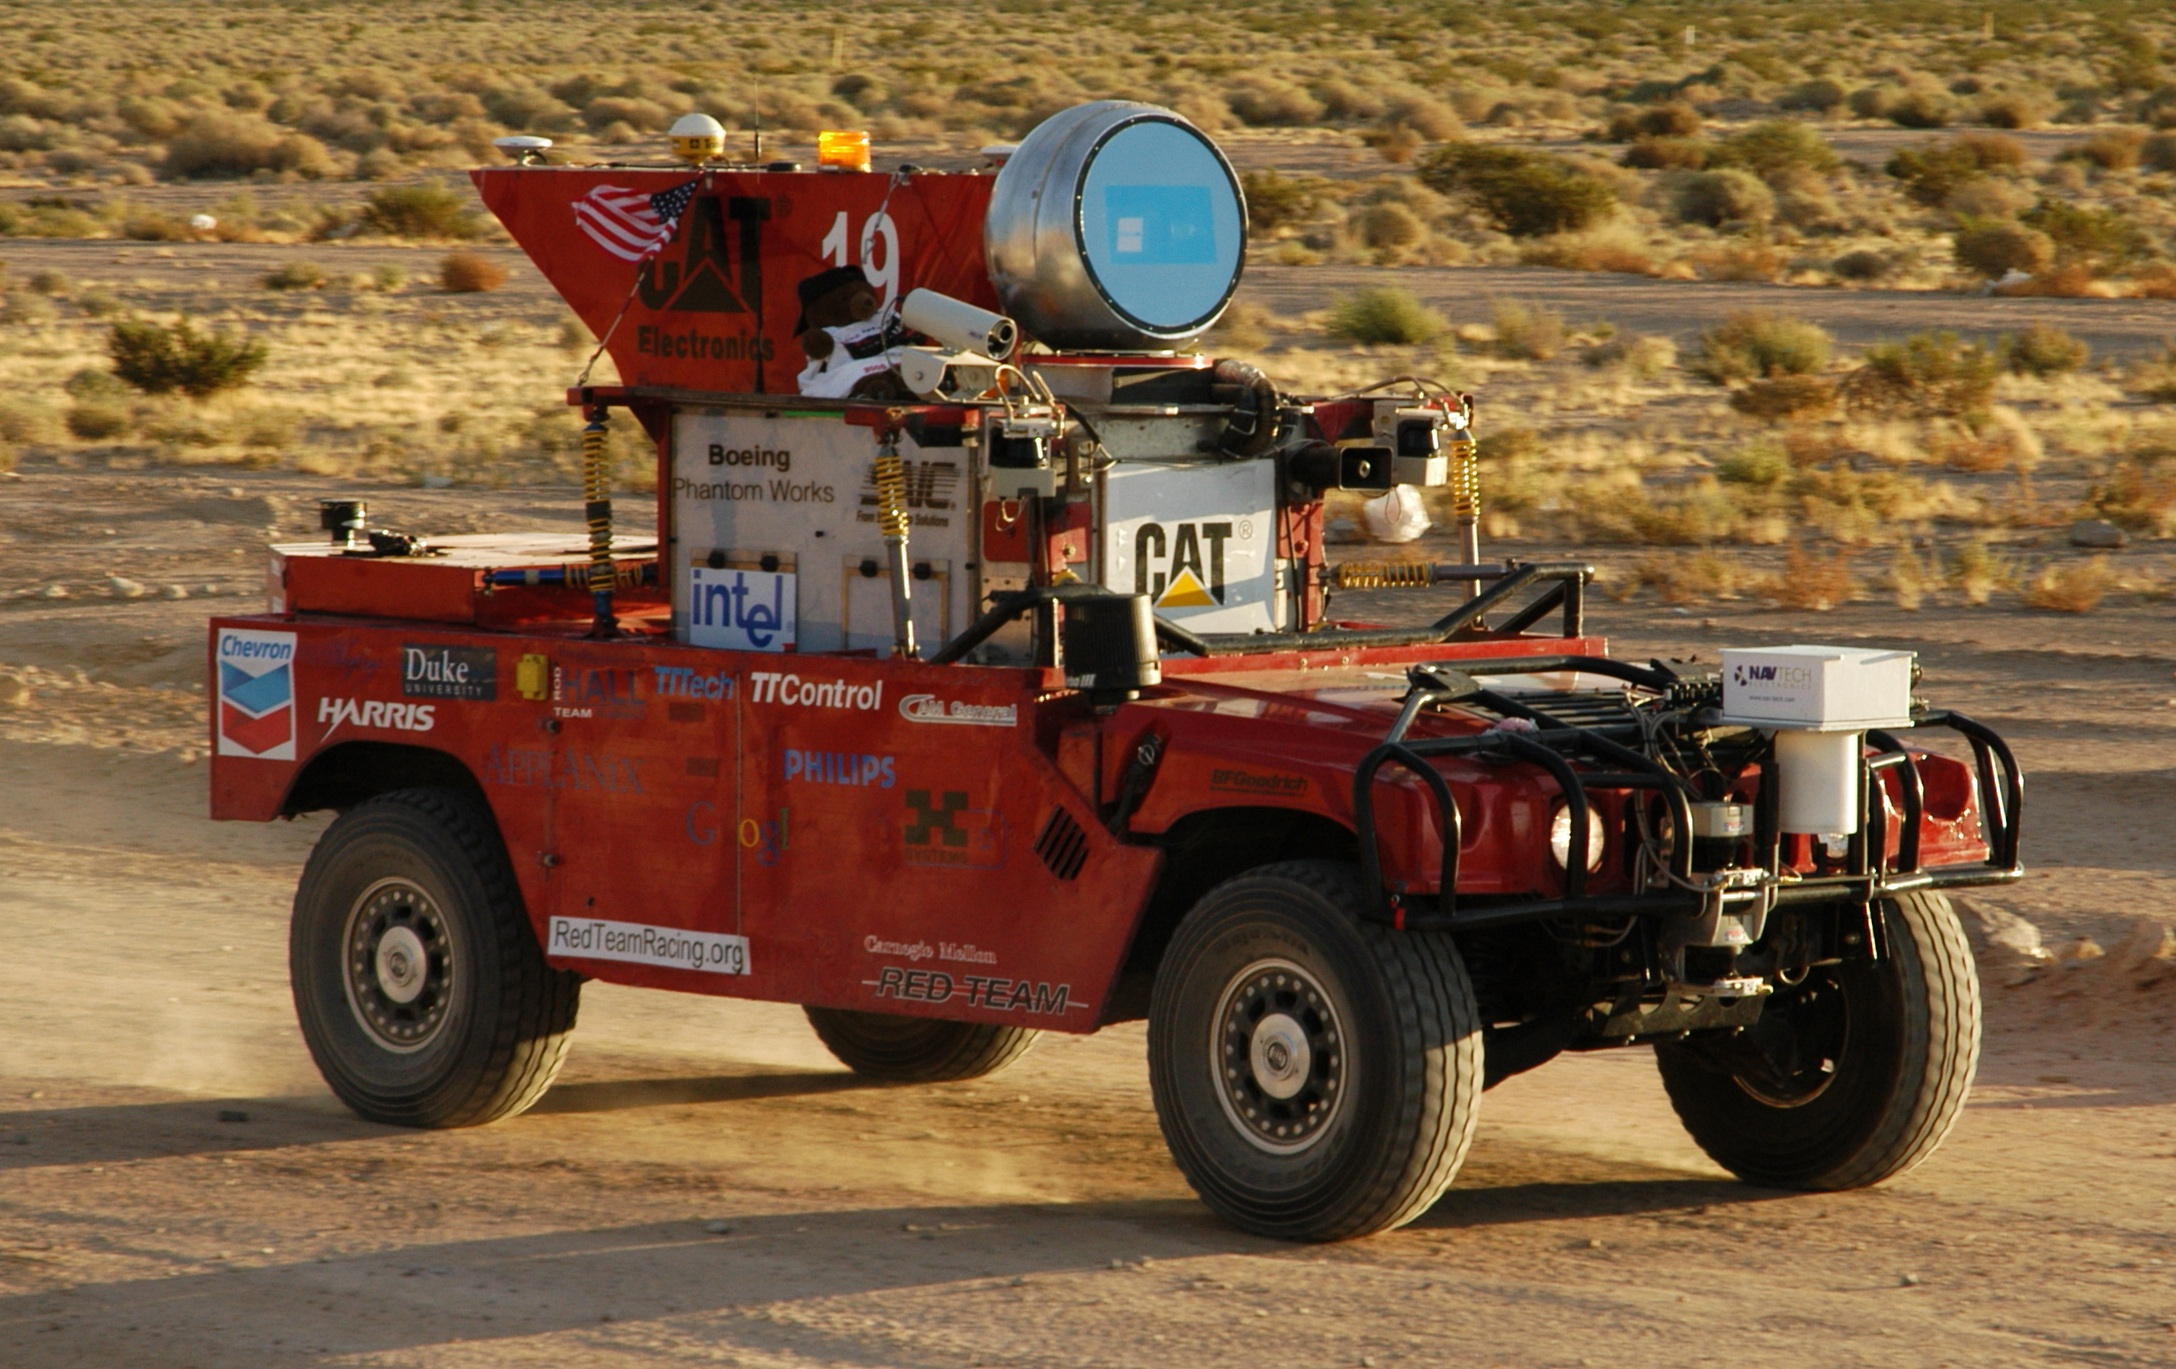
\includegraphics[width=\textwidth]{Sandstorm}
		    \end{subfigure}
		    \\~\\
		    \begin{subfigure}[b]{0.4\textwidth}
		      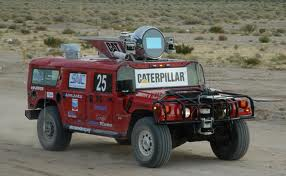
\includegraphics[width=\textwidth]{h1ghlander}
		    \end{subfigure}
		    ~
		    \begin{subfigure}[b]{0.4\textwidth}
		      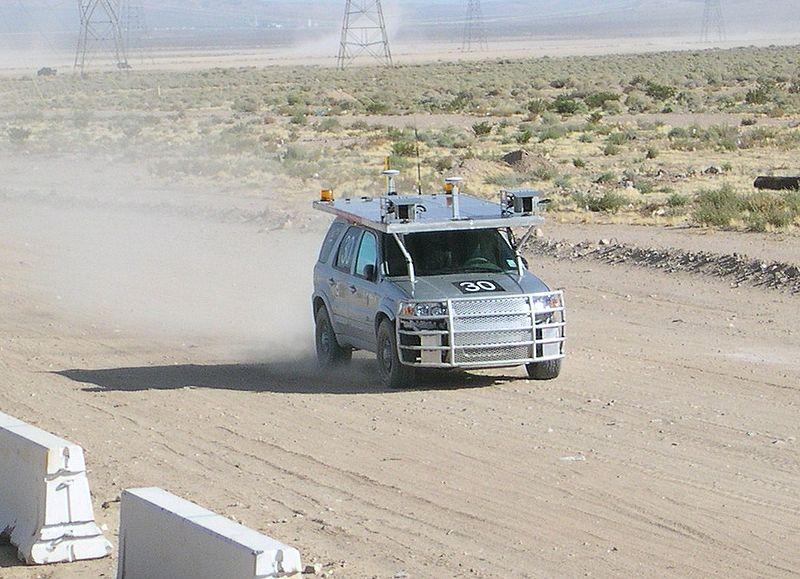
\includegraphics[width=\textwidth]{kat5}
		    \end{subfigure}
		    \\~\\
		    \begin{subfigure}[b]{0.4\textwidth}
		      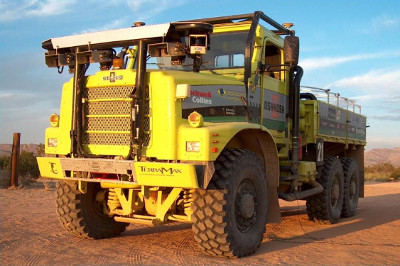
\includegraphics[width=\textwidth]{terramax}
		    \end{subfigure}
	    \end{figure}
	  \end{block}
	  }
	  \only<5>{
	  \begin{block}{DARPA's Urban Challenge}
	    \begin{figure}[t]
		    \centering
		    \begin{subfigure}[b]{0.4\textwidth}
		      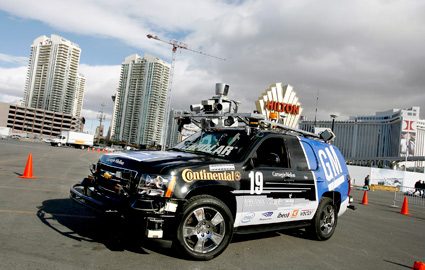
\includegraphics[width=\textwidth]{boss}
		    \end{subfigure}
		    ~
		    \begin{subfigure}[b]{0.4\textwidth}
		      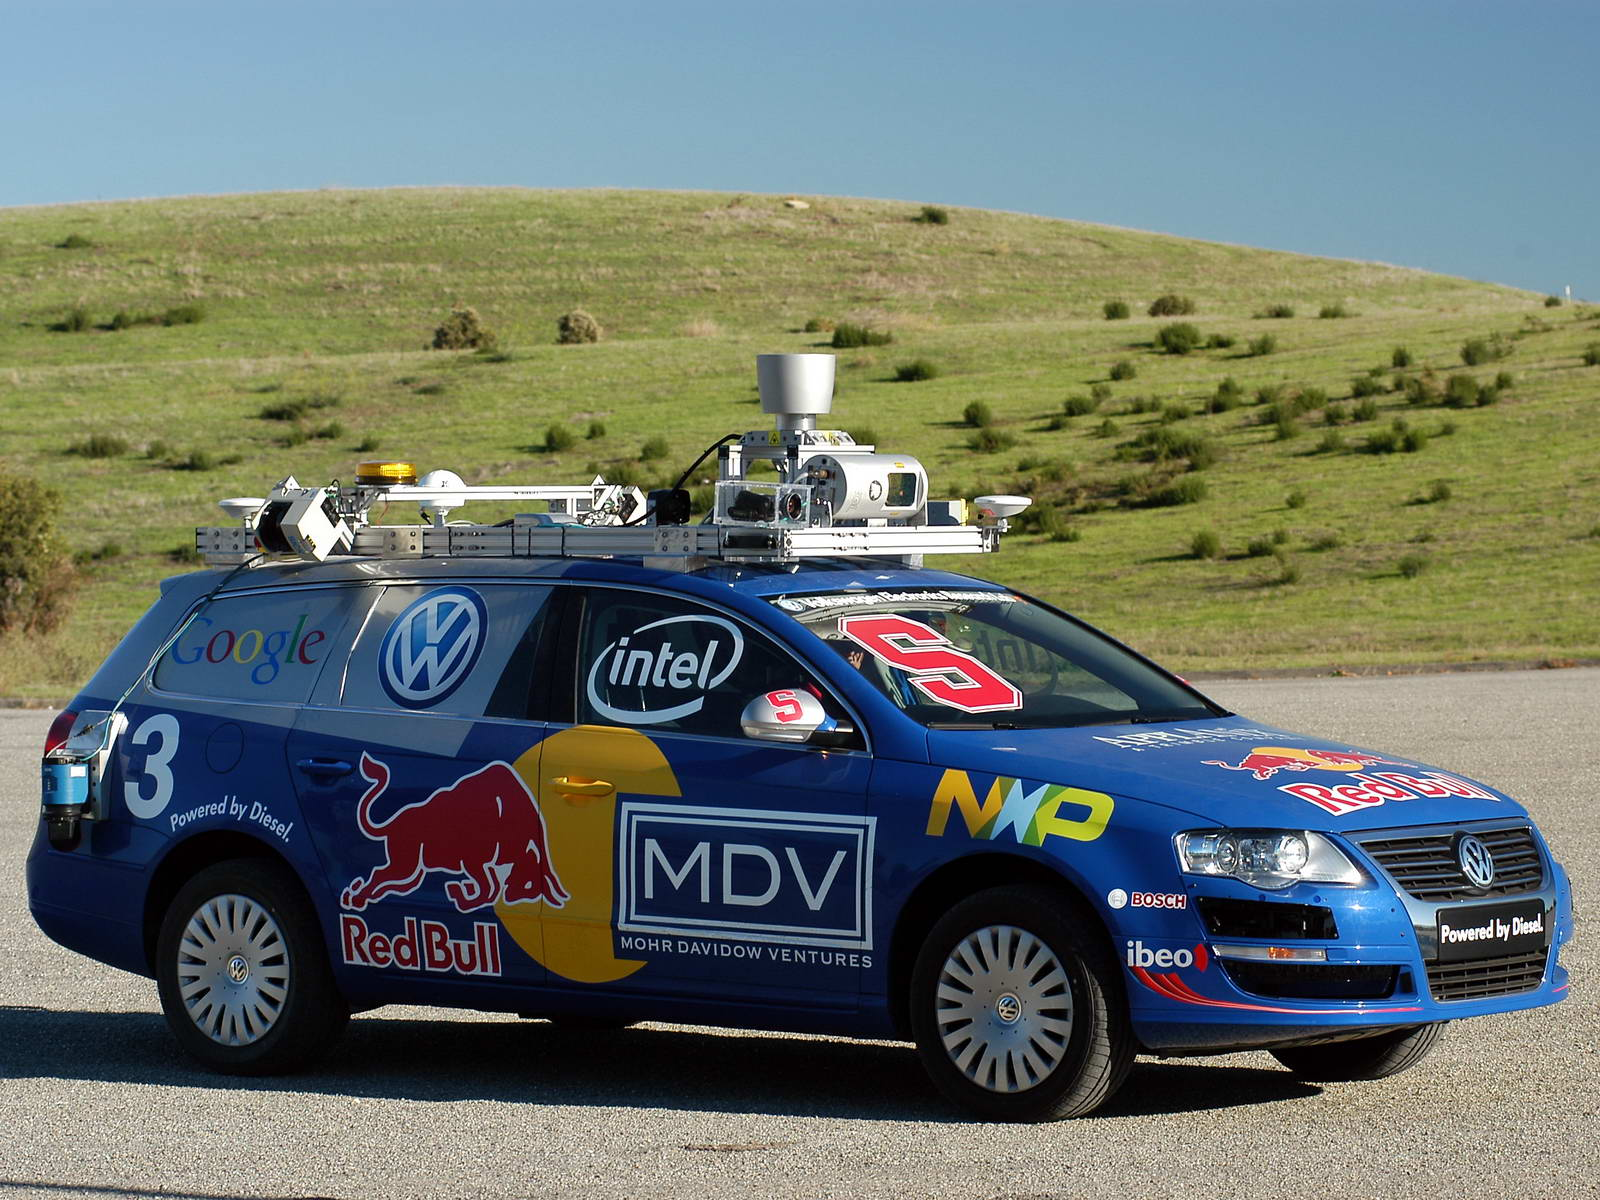
\includegraphics[width=\textwidth]{junior}
		    \end{subfigure}
		    \\~\\
		    \begin{subfigure}[b]{0.4\textwidth}
		      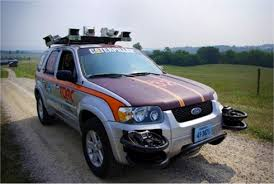
\includegraphics[width=\textwidth]{odin}
		    \end{subfigure}
		    ~
		    \begin{subfigure}[b]{0.4\textwidth}
		      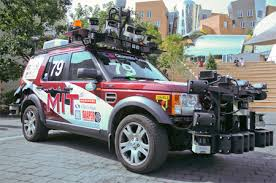
\includegraphics[width=\textwidth]{talos}
		    \end{subfigure}
		    \\~\\
		    \begin{subfigure}[b]{0.4\textwidth}
		      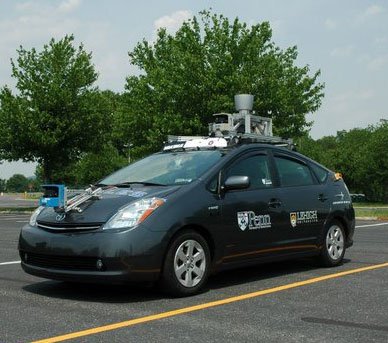
\includegraphics[width=\textwidth]{littleben}
		    \end{subfigure}
		    ~
		    \begin{subfigure}[b]{0.4\textwidth}
		      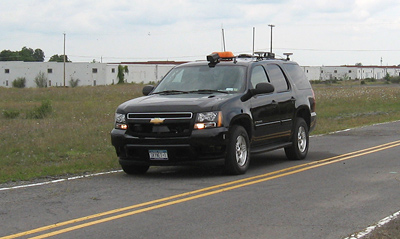
\includegraphics[width=\textwidth]{skynet}
		    \end{subfigure}

	    \end{figure}
	  \end{block}
	  }
	  \only<6>{
	  \begin{block}{Korean Autonomous Vehicle Competition (AVC)}
	    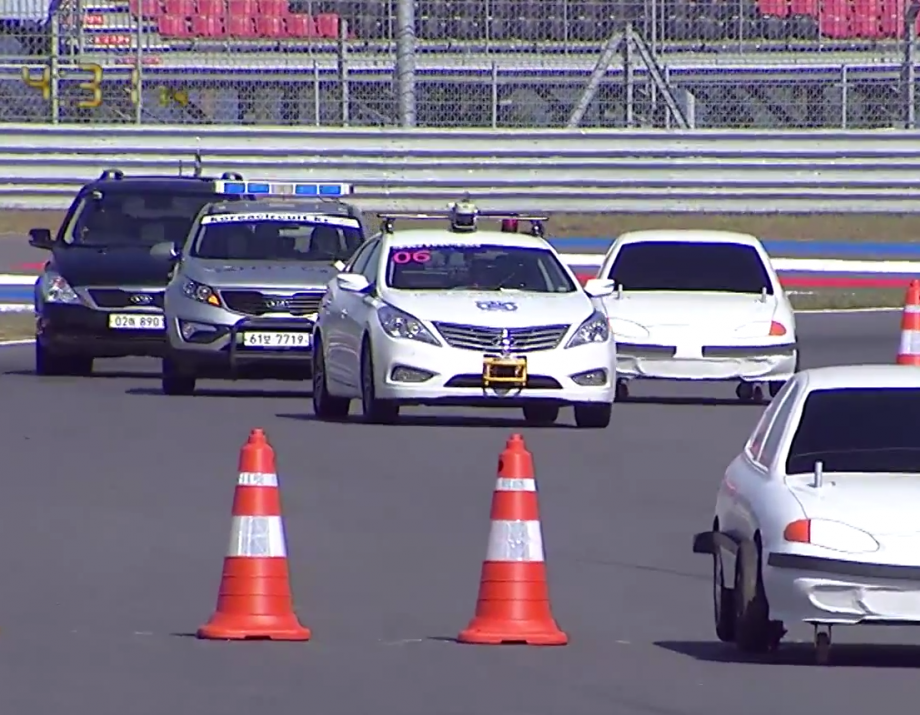
\includegraphics[width=\textwidth]{kavc}
	  \end{block}
	  }
	\end{overlayarea}
      \end{center}
    \end{columns}
    
    \note {
    \begin{itemize}
      \item From 1987 to 1995, the EC EUREKA Prometheus Project conducted research on autonomous vehicles. Among its culmination points were the twin robot vehicles VITA-2 and VaMP, driving long distances in heavy traffic.
      \item In 1996, the ARGO project modified a Lancia Thema to follow the lane marks in an unmodified highway \citep{Broggi1999}. The culmination of the project was a journey of 1,900\,km over six days on the motorways of northern Italy, with an average speed of 90 km/h. The car operated in fully automatic mode for the 94\% of its journey, with the longest automatic stretch being 55\,km. The vehicle had only two grayscale low-cost video cameras on board and used stereoscopic vision algorithms to understand its environment. 
      \item In 2004, DARPA's Grand Challenge was held in the Mojave Desert region of the United States, along a 240\,km route. This competition consisted on an autonomous vehicles race that must reach to the goal without human intervention and using just a listing of check points between the start and the finish line. None of the robot vehicles finished the route.
      \item In 2005, a second competition was held \citep{Buehler2007}. This time, five vehicles successfully completed the course:
      \begin{itemize}
      \item \emph{Stanley} \citep{thrun2006stanley}, from Standford University.
      \item \emph{Sandstorm} and \emph{H1ghlander} \citep{urmson2004high}, from the Carnegie Mellon University.
      \item \emph{Kat-5} \citep{trepagnier2006kat}, from the Gray Insurance Company.
      \item \emph{TerraMax} \citep{ozguner2004team}, from the Oshkosh Truck Corporation.
      \end{itemize}
      \item In 2007, the third driverless car competition of the DARPA Grand Challenge \citep{Buehler2009}, more known as the DARPA Urban Challenge, was held in Victorville, California. This time, six teams successfully finished the entire course:
      \begin{itemize}
      \item \emph{Boss} \citep{Urmson2008}, from the Carnegie Mellon University.
      \item \emph{Junior} \citep{montemerlo2008junior}, from Standford University.
      \item \emph{Odin} \citep{Bacha2008}, from Virginia Tech.
      \item \emph{Talos} \citep{leonard2007team}, from the Massachusetts Institute of Technology.
      \item \emph{Little Ben} \citep{bohren2008little}, from University of Pennsylvania.
      \item \emph{Skynet} \citep{miller2008team}, from Cornell University.
      \end{itemize}
      \item In 2010, 2012 and 2013, the Korean Autonomous Vehicle Competition (AVC) took place.
    \end{itemize}
    }
  \end{frame}

  \begin{frame}{Autonomous vehicles review}
    \begin{columns}[T] % the "c" option specifies center vertical alignment
      \column{.5\textwidth} % column designated by a command
      \footnotesize
      \begin{itemize}
	\item<1-> \textbf{(2010)} VIAC Challenge.
	\item<3-> \textbf{(2011)} WildCat Project.
	\item<4-> \textbf{(2011)} AutoNOMOS Group.
	\item<5-> \textbf{(2012)} Shelley.
	\item<6-> \textbf{(February 2013)} RobotCar project.
	\item<7-> \textbf{(July 2013)} BRAiVE.
	\item<8-> \textbf{(Nowadays)} Many working prototypes.
      \end{itemize}  
      \column{.5\textwidth}
      \begin{center}
	\vskip -1cm
       	\begin{overlayarea}{\textwidth}{\textheight}
	  \only<1-2>{
	  \begin{block}{VIAC Challenge}
	    \begin{itemize}
	    \item<1-> From Italy to China.
	    \item<1-> 100 day, 15,900\,km.
	    \item<2-> Four autonomous vehicles.
	    \item<2-> Limited human intervention.
	    \end{itemize}
	    \begin{center}
	      \includegraphics<1>[width=0.8\textwidth]{viacMap}
	      \includegraphics<2>[width=0.8\textwidth]{viacCars}
	    \end{center}

	  \end{block}
	  }
	  \only<3>{
	  \begin{block}{WildCat Project}
	    \begin{itemize}
	      \item Bowler Wildcat.
	      \item Oxford University.
	    \end{itemize}
	    \begin{center}\includegraphics<1->[width=\textwidth]{wildcat}\end{center}
	  \end{block}
	  }
	  \only<4>{
	  \begin{block}{AutoNOMOS Group}
	    \begin{itemize}
	      \item Spirit of Berlin.\\
	      \begin{center}\includegraphics<1->[width=0.5\textwidth]{spiritofberlin}\end{center}
	      \item MadeInGermany.\\
	      \begin{center}\includegraphics<1->[width=0.5\textwidth]{madeingermany}\end{center}
	    \end{itemize}
	  \end{block}
	  }
	  \only<5>{
	  \begin{block}{Shelley}
	    \begin{itemize}
	      \item More than 160\,km/h
	    \end{itemize}
	    \begin{center}\includegraphics<1->[width=\textwidth]{shelley}\end{center}
	  \end{block}
	  }
	  \only<6>{
	  \begin{block}{RobotCar project}
	    \begin{itemize}
	      \item Oxford University.
	      \item Switches from manual to autopilot on learned routes.
	    \end{itemize}
	    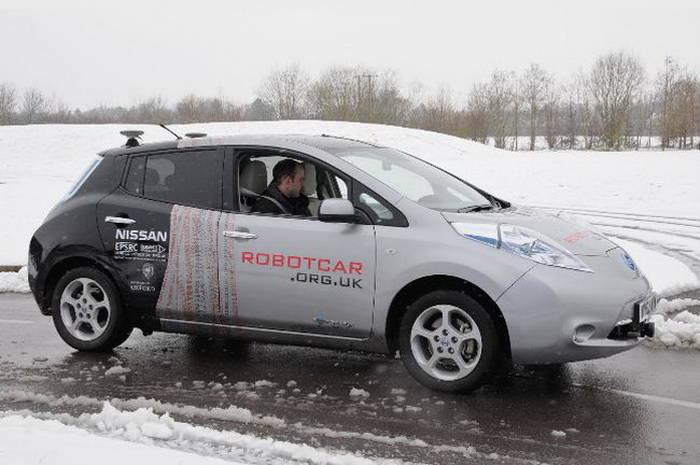
\includegraphics[width=\textwidth]{robotcar}
	  \end{block}
	  }
	  \only<7>{
	  \begin{block}{BRAiVE}
	    \begin{itemize}
	      \item Vislab.
	      \item Moved on a mixed traffic route open to public traffic.
	    \end{itemize}
	    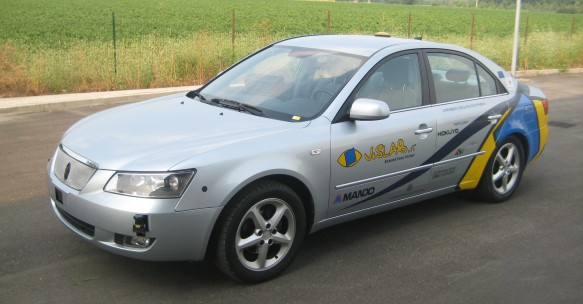
\includegraphics[width=\textwidth]{BRAiVE}
	  \end{block}
	  }
	  \only<8>{
	  \begin{block}{Many working prototypes}
	    \begin{figure}[t]
	      \centering
	      \begin{subfigure}[b]{0.2\textwidth}
		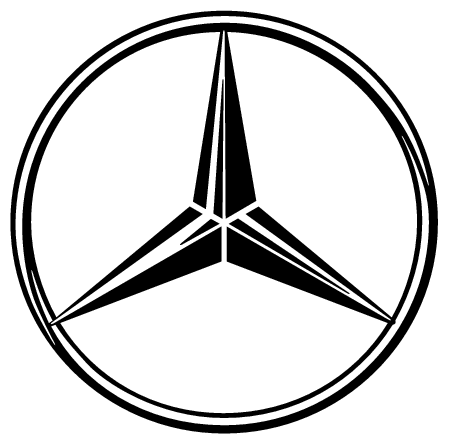
\includegraphics[width=\textwidth]{mercedes_benz}
	      \end{subfigure}
	      ~
	      \begin{subfigure}[b]{0.2\textwidth}
		
\includegraphics[width=\textwidth]{gm}
	      \end{subfigure}
	      ~
	      \begin{subfigure}[b]{0.2\textwidth}
		
\includegraphics[width=\textwidth]{continental}
	      \end{subfigure}
	      \\~\\
	      \begin{subfigure}[b]{0.2\textwidth}
		
\includegraphics[width=\textwidth]{autoliv}
	      \end{subfigure}
	      ~
	      \begin{subfigure}[b]{0.2\textwidth}
		
\includegraphics[width=\textwidth]{bosch}
	      \end{subfigure}
	      ~
	      \begin{subfigure}[b]{0.2\textwidth}
		
\includegraphics[width=\textwidth]{nissan}
	      \end{subfigure}
	      \\~\\
	      \begin{subfigure}[b]{0.2\textwidth}
		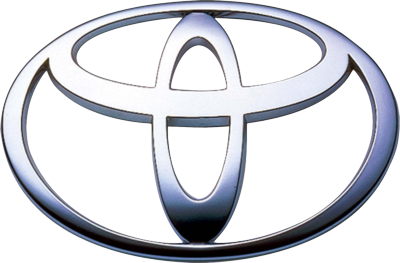
\includegraphics[width=\textwidth]{toyota}
	      \end{subfigure}
	      ~
	      \begin{subfigure}[b]{0.2\textwidth}
		
\includegraphics[width=\textwidth]{audi}
	      \end{subfigure}
	      ~
	      \begin{subfigure}[b]{0.2\textwidth}
		
\includegraphics[width=\textwidth]{vislab_logo}
	      \end{subfigure}
	      \\~\\
	      \begin{subfigure}[b]{0.2\textwidth}
		
\includegraphics[width=\textwidth]{oxforduni_logo}
	      \end{subfigure}
	      ~
	      \begin{subfigure}[b]{0.2\textwidth}
		
\includegraphics[width=\textwidth]{google}
	      \end{subfigure}
	    \end{figure}
	  \end{block}
	  }
	\end{overlayarea}
      \end{center}
    \end{columns}
    
    \note {
    \begin{itemize}
      \item In 2010, inside the VIAC Challenge, four autonomous vehicles drove from Italy to China on a 100-day 15,900\,km trip with only limited human intervention (in traffic jams and when passing toll stations). At the time, this was the longest-ever journey conducted by an unmanned vehicle \citep{Broggi2010VIAC}.
      \item In 2011, under the Oxford University's WildCat Project, a Bowler Wildcat based prototype is capable of autonomous operation using a flexible and diverse sensor suite.
      \item In 2011, the Freie Universität Berlin, Led by the AutoNOMOS group, developed two autonomous cars - \emph{Spirit of Berlin} \citep{berlin2007spirit} and \emph{MadeInGermany} \citep{gohring2013semi} - to drive in the innercity traffic of Berlin in Germany. They were able to handle intercity traffic, traffic lights and roundabouts between the International Congress Centrum and the Brandenburg Gate.
      \item In 2012, Stanford's Dynamic Design Lab, in collaboration with the Volkswagen Electronics Research Lab, produced Shelley, an Audi TTS designed for high speed (greater than 160\,km/h) on a racetrack course.
      \item In February 2013, Oxford University unveiled the RobotCar UK project, an inexpensive autonomous car capable of quickly switching from manual driving to autopilot on learned routes.
      \item In July 2013, Vislab worldpremiered BRAiVE, a vehicle that moved autonomously on a mixed traffic route open to public traffic \citep{grisleri2010braive}.
      \item Currently, many major companies and research organizations have developed working prototype autonomous vehicles, including Mercedes-Benz, General Motors, Continental Automotive Systems, Autoliv Inc., Bosch, Nissan, Toyota, Audi, Vislab (University of Parma), Oxford University and Google.
    \end{itemize}
    }
  \end{frame}
  
  \begin{frame}{Obstacle detection}
    We can divide object tracking methods into two subcategories:
    \begin{itemize}
      \item \emph{2.5D Solutions:} Different approaches:
      \begin{itemize}
	\item \emph{Use of the 3D point as feature.} \cite{franke20056d}
	\item \emph{Dynamic stixels.} \cite{badino2009stixel, pfeiffer2011towards, pfeiffer2013exploiting, benenson2011stixels, benenson2012pedestrian, benenson2012fast}
	\item \emph{Tracked image features.} \cite{barth2009estimating}
	\item \emph{Sensor fusion.} \cite{wu2009collision}
	\item \emph{Occupancy grids.} \cite{danescu2012particle}
      \end{itemize} 
      \item \emph{3D Solutions}
      \begin{itemize}
	\item \emph{Octree connected cubes.} \cite{broggi2013}
	\item \emph{Adjacent stacks of cells} \cite{Moravec96robotspatial}
      \end{itemize}
    \end{itemize}
    
    \note{
    Based on how much information they use, we can divide object tracking methods into two subcategories:
    \begin{itemize}
      \item \emph{2.5D Solutions:} They do not make use of the complete information provided by 3D points. Instead of that, they tend to use elevation maps composed of uniform size cells. Each cell just stores occupancy and height information. This is the kind of methods that, as described before, usually consider obstacles as being in contact with a flat ground.
      In these methods, tracking is performed before the complete reconstruction is done, in an intermediate point based on an specific feature. Depending on the feature used, we distinguishing different approaches:
      \begin{itemize}
	\item \emph{Use of the 3D point as feature.} An example of this is the so called 6D vision \citep{franke20056d}, in which the 3D stereo vision extracted information is combined with an efficient implementation of an optical flow in the image space based on a \ac{GPU}. Relevant points are tracked using a Kalman filter.
	\item \emph{Dynamic stixels.} This approach has been longer discussed in section \ref{ch:chapter00_02_04}.
	\item \emph{Tracked image features.} An example is the work by \cite{barth2009estimating}. There, obstacles are represented as a rigid 3D point set which are tracked in terms of feature displacements and depth measurements.
	\item \emph{Sensor fusion.} \cite{wu2009collision} reconstruct the objects as cuboids from a stereo point cloud. In this process, position and speed values are improved to a very accurate value by the use of a radar along with stereo.
	\item \emph{Occupancy grids.} This is a very popular choice for tracking. An occupancy grid is a probabilistic map of the driving environment, which encodes the past and present knowledge from sensor data, and which can be updated dynamically when new information is available. These occupancy grids can be cartesian, with rectangular cells, polar, or even a relation between columns in an image and the disparity. An example of this is the method by \cite{danescu2012particle}, which has inspired part of the work described in chapter \ref{ch:chapter05}.
	Another advantage of the model based on an occupancy grid is that it makes easier a collaborative update of the grid, which allows the usage of data from several sensors and observers. Another simple example of occupancy grid is that described in chapter \ref{ch:chapter07}.
      \end{itemize} 
      \item \emph{3D Solutions:} Usually based on complex grid maps that use complete 3D information. Again, depending on how this grid is represented, we find 
      \begin{itemize}
	\item \emph{Octree connected cubes.} An example is the work by \cite{wurm2010octomap} or \cite{broggi2013}.
	\item \emph{Adjacent stacks of cells}, as described in \cite{Moravec96robotspatial} 
      \end{itemize}
    \end{itemize}
    }
  \end{frame}

  \begin{frame}{Path planning}
    \begin{itemize}
      \item Classical methods \citep{hwang1992gross}
      \item Heuristic methods \citep{masehian2007classic}
      \item SVM based methods
      \begin{itemize}
       \item Global
	 \begin{itemize}
	  \item \cite{miura2006support}
	  \item \cite{yang2012safe}
	 \end{itemize}
       \item Local
	\begin{itemize}
	  \item \cite{sarkar2008mobile}
	  \item \cite{tennety2009support}
	  \item \cite{qingyang2012local}
	\end{itemize}
      \end{itemize}
    \end{itemize}
    
    \note{
      About classical methods, in general they can be considered as variations of some general approaches: Roadmap, Cell Decomposition, Potential Fields and Mathematical Programming. These methods are not mutually exclusive; in fact, a lot of approaches use combinations of them. A review of some classical methods can be checked out in \cite{hwang1992gross}.
 
      About heuristic methods, these are the answer given by researchers to the limitations of the classic methods. The most representative methods inside this classification are Probabilistic Roadmaps (PRM) \citep{kavraki1996probabilistic}, Rapidly Exploring Random Trees (RRT) \citep{lavalle2000rapidly}, Level set \citep{sethian1999level}, Linguistic Geometry (LG) \citep{stilman1993network}, Simulated Annealing (SA) \citep{zhu2006robot}, Artificial Neural Network (ANN) \citep{hossain2012real}, Genetic Algorithms (GA) \citep{zhang2007evolutionary}, Particle Swarm Optimization (PSO) \citep{chen2006smooth}, Ant Colony (ACO) \citep{mou2008modified} and its variants, like the RNA algorithm described in \cite{zhu2011new}, Stigmergy \citep{cazangi2006evolutionary}, Wavelet Theory \citep{doh2005systematic}, Fuzzy Logic (FL) \citep{kladis2011energy} and Tabu Search (TS) \citep{nguyen2012multi}. For more information, the review in \cite{masehian2007classic} can be checked.
      
      Global:
      In the work presented by \cite{miura2006support}, navigation is planned in environments in which the obstacles are known. Obstacles are randomly labeled into two classes: positive or negative. Using these two classes, a \ac{SVM} is trained and the decision boundary is used as a path. To increase the efficiency, a set of fake obstacles (guide samples) is generated at both sides of the current and goal position, as well as in parallel to the line that joins both points (nominal line), with the objective of helping the \ac{SVM} to find a feasible path.
      \cite{yang2012safe}. In their work, a preprocessing step is used in which the Voronoi Diagram is generated using the obstacles in the map. That diagram is used to select the best path between the starting point of the robot and the goal. The path obtained using Voronoi is not smooth, so the \ac{SVM} is used to make this path smoother. The \ac{SVM} is trained using a dataset in which the sites that generated the Voronoi edges are classified as positive or negative depending on their position (left / right) regarding to the previously obtained path. The decision boundary of this \ac{SVM} will be the final path used.
      
      Local:
      In \cite{sarkar2008mobile, tennety2009support}, authors divide the whole set of objects in the map into two classes and the \ac{SVM} is used to determine the maximum margin hyperplane between the data sets belonging to the two classes. Data is assigned to one or another class depending on whether the points are on the left or on the right side of the robot. Once the initial labels are assigned, further classification is done using the k-nearest neighbor algorithm, with k=1.
      \cite{qingyang2012local}, that uses a path subdivision method and a \ac{SVM}. They use topological maps of local environments which are extracted with little expanded nodes. Next, candidate routes are optimized using the Support Vector Machine, where the candidate routes boundary points are defined as positive and negative samples. They also extend the original \ac{SVM} \citep{cortes1995support} in order to satisfy extra constraints such as vehicle position and heading.
    }
  \end{frame}
  
    \begin{frame}{Local planning}
    \begin{itemize}
      \item \cite{werling2010optimal}
      \item \cite{thrun2006stanley}
      \item \cite{chu2012local}
    \end{itemize}
     
    \note{
      \begin{itemize}
	\item In \cite{werling2010optimal}, long term objectives are performed, like speed keeping, merging, following, stopping. This is done through optimal control strategies within the Fren\'et frame of the street.
	\item In \cite{thrun2006stanley}, lateral offset is defined as the perpendicular to an established base trajectory. This allows the vehicle driving along the road parallel to this trajectory. In order to select the optimal path, the cost function penalizes passing over obstacles and the distance respect to the center of the current road.
	\item In \cite{chu2012local}, also a set of candidate paths are generated, with endpoints in fixed positions at different offsets respect to the base frame, but they do not set this base frame in the center of the road, since it could be dangerous when computing the costs at certain scenarios. Instead of that, they use a security cost for each candidate path. Security of the path is computed by blurring the binary data of the obstacles. They also have into account certain criteria, as the smoothness cost or the path consistency between iterations.
      \end{itemize}
    }
  \end{frame}
  
  \subsection{Testing platform}
  \begin{frame}{Testing platform}
    These algorithms are intended to be used in Verdino.
    \begin{itemize}
     \item<1-> Prototype developed by GRULL, Universidad de La Laguna.
     \item<2-> It will transport people around a bioclimatic urbanization in the ITER facilities.
     \item<3-> A golf cart has been modified to be used as an unmanned vehicle.
    \end{itemize}

    \begin{center}
      \includegraphics<1-1>[height=.3\columnwidth]{verdino}
      \includegraphics<2-2>[height=.3\columnwidth]{iter}
      \includegraphics<3-4>[height=.3\columnwidth]{NV_TXT2}
      \includegraphics<4-4>[height=.3\columnwidth]{verdino}
    \end{center}
  \end{frame}
  
  \begin{frame}{Actuators}
    \begin{columns}[c] % the "c" option specifies center vertical alignment
      \column{.5\textwidth} % column designated by a command
      \begin{itemize}
	\item<1-> Steering system.      
	\item<2-> Braking system.
	\item<3-> Speed system.
	\item<4-> Safety switch.
      \end{itemize}  
      \column{.5\textwidth}
      \begin{center}
	\includegraphics<1-1>[width=\textwidth]{steering}
	\includegraphics<2-2>[width=\textwidth]{braking}
	\includegraphics<3-3>[width=\textwidth]{speedControl}
	\includegraphics<4-4>[width=\textwidth]{panicbutton}
      \end{center}
    \end{columns}
    
    \note {
    \begin{itemize}
      \item Steering system: we tied the original steering to a DC motor controlled by a PID.
      \item Braking system: Controlled through a pneumatic system, composed by a cylinder, a commutation valve, two flow controllers and an air compressor. The pneumatic cylinder acts over the brake cables, that make pressure over the brake drums. A compressor gives the air pressure needed for this process.
      \item Speed system: A microcontroller generates three different signals, that simulate the original devices installed in the vehicle. These correspond to a switch relay, which turns on the motor when the user pushes the acceleration pedal; the sense of speed (forward or backward); and the desired voltage
      \item Safety switch: Allows changing between automatic and manual behavior. When switched off, the vehicle behaves as it was before the modifications.
    \end{itemize}
    }
  \end{frame}

  \begin{frame}{Sensors}
    \begin{columns}[c] % the "c" option specifies center vertical alignment
      \column{.5\textwidth} % column designated by a command
      \begin{itemize}
	\item<1-> Localization sensors.      
	\begin{itemize}
	  \item<3-> Odometry.      
	  \item<4-> IMU.
	  \item<5-> Differential GPS.
	\end{itemize}  
	\item<2-> Navigation sensors.	
	\begin{itemize}
	  \item<6-> LIDAR.      
	  \item<7-> IR cameras.
	  \item<8-> Visible cameras.
	\end{itemize}
      \end{itemize}  
      \column{.5\textwidth}
      \begin{center}
	\includegraphics<3-3>[width=\textwidth]{odometry}
	\includegraphics<4-4>[width=\textwidth]{imu}
	\includegraphics<5-5>[width=\textwidth]{dgps}
	\includegraphics<6-6>[width=\textwidth]{lidar}
	\includegraphics<7-7>[width=\textwidth]{ircameras}
	\includegraphics<8-8>[width=\textwidth]{visiblecamera}
      \end{center}
    \end{columns}
    
    \note {
    \begin{itemize}
      \item \emph{Odometry}: This system measures the independent movement of the two rear wheels, which are attached to an optical encoder. This allows computing the position, orientation and speed of the prototype incrementally.
      \item \emph{\acf{IMU}}: It is comprised by 9 sensors (3 accelerometers, 3 gyroscopes and 3 magnetometers), which are fused in real time in order to get the three-dimensional orientation of the vehicle. The model of the sensor is a \emph{Xsens Mti}.
      \item \emph{\acf{DGPS}}: Allows positioning the vehicle with centimetric accuracy. It is composed by two different devices, the reference station, which is fixed in a known place, and the rover station, which is installed on the vehicle. The model used is a \emph{JAVAD GNSS Triumph-1}, which has an horizontal precision below 1\,cm and a vertical precision around 1.5\,cm using \ac{DGPS}, at a frequency of $5\,Hz$.
      \item \emph{\acf{LIDAR}}: These are used also for localization purposes. Each of those sensors is able to detect the objects in the way of the vehicle, at the plane in which the sensor is mounted. The advantages of these sensors are that they have a high speed and precision. However, they are just able to detect obstacles that crosses the plane defined by the sensor. Because of this, we have equipped the vehicle with 5 \acp{LIDAR}. Two of them are located at the same plane in the front corners of the vehicle, at a height of 50\,cm. Each of these covers an angle of 270\textdegree. Another is located in the front side of the vehicle, at a height of 20\,cm, slightly tilted upwards, in order to detect the small obstacles or non traversable areas. Another is in the top of the vehicle, also in the front side of the vehicle, tilted to the ground and covering the blind areas left by the other sensors. Finally, the last sensor is situated in the back side of the vehicle, and it is used for backwards maneuvers. The used sensors are of the model \emph{SICK LMS 100} and \emph{SICK LMS 111}, allowing a maximal detection distance of 20\,m, a precision of 10-35\,mm, a maximal angular resolution of 0.25\textdegree and a maximal rate of $50\,Hz$.
      \item \emph{IR cameras}: Infrared cameras are used to detect pedestrians or animals based on their temperature. We have a pair of them installed on a Pan-Tilt system attached to the top front side of the vehicle. The model used is a \emph{MobiR\textregistered~M3}, which is able to detect objects in the range $8\sim14\mu m$, at a resolution of $160 \times 120\,px$.
      \item \emph{Visible cameras}: A set of three cameras is also installed in a pan-tilt structure. These are used for the detection and tracking of the objects, which is one of the goals of this thesis. Also, they are currently being used for the detection of the borders of the road. The model of the cameras is a \emph{GoPro\textregistered Hero 3 silver edition}, with a $1920 \times 1080 \, px$ maximal video resolution and a 170\textdegree field of view at a maximal rate of 60\,fps.
    \end{itemize}
    }
  \end{frame}
  
  \begin{frame}{Control}
    \begin{columns}[c] % the "c" option specifies center vertical alignment
      \column{.5\textwidth} % column designated by a command
      \begin{itemize}
	\item<1-> Onboard computer.   
	\begin{itemize}
	  \item<2-> i7-3770K.      
	  \item<2-> 16 Gb RAM DDR3.
	  \item<2-> SSD Storage.
	\end{itemize}	
	\item<3-> Low-level control.
      \end{itemize}  
      \column{.5\textwidth}
      \begin{center}
	\includegraphics<1->[width=\textwidth]{onboard}
      \end{center}
    \end{columns}
    
    \note {
    The vehicle is controlled, at high level, by an on board computer equipped with an \emph{i7-3770K} processor, 16\,Gb of \emph{RAM DDR-3} memory and a \emph{SSD} storage. At low level, a set of own developed electronic devices receive commands from the computer and transform them into the right signal, understandable by the actuators described before.
    }
  \end{frame}
  